%% BioMed_Central_Tex_Template_v1.06
%%                                      %
%  bmc_article.tex            ver: 1.06 %
%                                       %

%%IMPORTANT: do not delete the first line of this template
%%It must be present to enable the BMC Submission system to
%%recognise this template!!

%%%%%%%%%%%%%%%%%%%%%%%%%%%%%%%%%%%%%%%%%
%%                                     %%
%%  LaTeX template for BioMed Central  %%
%%     journal article submissions     %%
%%                                     %%
%%          <8 June 2012>              %%
%%                                     %%
%%                                     %%
%%%%%%%%%%%%%%%%%%%%%%%%%%%%%%%%%%%%%%%%%


%%%%%%%%%%%%%%%%%%%%%%%%%%%%%%%%%%%%%%%%%%%%%%%%%%%%%%%%%%%%%%%%%%%%%
%%                                                                 %%
%% For instructions on how to fill out this Tex template           %%
%% document please refer to Readme.html and the instructions for   %%
%% authors page on the biomed central website                      %%
%% http://www.biomedcentral.com/info/authors/                      %%
%%                                                                 %%
%% Please do not use \input{...} to include other tex files.       %%
%% Submit your LaTeX manuscript as one .tex document.              %%
%%                                                                 %%
%% All additional figures and files should be attached             %%
%% separately and not embedded in the \TeX\ document itself.       %%
%%                                                                 %%
%% BioMed Central currently use the MikTex distribution of         %%
%% TeX for Windows) of TeX and LaTeX.  This is available from      %%
%% http://www.miktex.org                                           %%
%%                                                                 %%
%%%%%%%%%%%%%%%%%%%%%%%%%%%%%%%%%%%%%%%%%%%%%%%%%%%%%%%%%%%%%%%%%%%%%

%%% additional documentclass options:
%  [doublespacing]
%  [linenumbers]   - put the line numbers on margins

%%% loading packages, author definitions

%\documentclass[twocolumn]{bmcart}% uncomment this for twocolumn layout and comment line below
\documentclass{bmcart}

%%% Load packages
%\usepackage{amsthm,amsmath}
%\RequirePackage{natbib}
%\RequirePackage[authoryear]{natbib}% uncomment this for author-year bibliography
%\RequirePackage{hyperref}
\usepackage[utf8]{inputenc} %unicode support
\usepackage[T1]{fontenc}
\usepackage{hyperref}
\usepackage{float}
\usepackage{cite}
\usepackage{nameref,hyperref}
\usepackage{graphicx}

\newfloat{suppfig}{tbh}{losf}
\floatname{suppfig}{\textbf{Supplementary Figure}}

%\usepackage[applemac]{inputenc} %applemac support if unicode package fails
%\usepackage[latin1]{inputenc} %UNIX support if unicode package fails


%%%%%%%%%%%%%%%%%%%%%%%%%%%%%%%%%%%%%%%%%%%%%%%%%
%%                                             %%
%%  If you wish to display your graphics for   %%
%%  your own use using includegraphic or       %%
%%  includegraphics, then comment out the      %%
%%  following two lines of code.               %%
%%  NB: These line *must* be included when     %%
%%  submitting to BMC.                         %%
%%  All figure files must be submitted as      %%
%%  separate graphics through the BMC          %%
%%  submission process, not included in the    %%
%%  submitted article.                         %%
%%                                             %%
%%%%%%%%%%%%%%%%%%%%%%%%%%%%%%%%%%%%%%%%%%%%%%%%%


\def\includegraphic{}


%%% Put your definitions there:
\startlocaldefs
\def\p{{\mathbf p}}
\def\q{{\mathbf q}}
\def\r{{\mathbf r}}
\def\l{{\mathbf l}}
\endlocaldefs


%%% Begin ...
\begin{document}

%%% Start of article front matter
\begin{frontmatter}

\begin{fmbox}
\dochead{SOFTWARE}

%%%%%%%%%%%%%%%%%%%%%%%%%%%%%%%%%%%%%%%%%%%%%%
%%                                          %%
%% Enter the title of your article here     %%
%%                                          %%
%%%%%%%%%%%%%%%%%%%%%%%%%%%%%%%%%%%%%%%%%%%%%%

\title{A new Sequence logo plot to highlight enrichment and depletion}

%%%%%%%%%%%%%%%%%%%%%%%%%%%%%%%%%%%%%%%%%%%%%%
%%                                          %%
%% Enter the authors here                   %%
%%                                          %%
%% Specify information, if available,       %%
%% in the form:                             %%
%%   <key>={<id1>,<id2>}                    %%
%%   <key>=                                 %%
%% Comment or delete the keys which are     %%
%% not used. Repeat \author command as much %%
%% as required.                             %%
%%                                          %%
%%%%%%%%%%%%%%%%%%%%%%%%%%%%%%%%%%%%%%%%%%%%%%

\author[
   addressref={aff1},                   % id's of addresses, e.g. {aff1,aff2}
   corref={aff1},                       % id of corresponding address, if any
   email={kkdey@uchicago.edu}   % email address
]{\inits{KKD}\fnm{Kushal K} \snm{Dey}}
\author[
   addressref={aff1},
   email={dyxie@uchicago.edu}
]{\inits{DX}\fnm{Dongyue} \snm{Xie}}
\author[
   addressref={aff1, aff2},
   email={mstephens@uchicago.edu}
]{\inits{MS}\fnm{Matthew} \snm{Stephens}}

%%%%%%%%%%%%%%%%%%%%%%%%%%%%%%%%%%%%%%%%%%%%%%
%%                                          %%
%% Enter the authors' addresses here        %%
%%                                          %%
%% Repeat \address commands as much as      %%
%% required.                                %%
%%                                          %%
%%%%%%%%%%%%%%%%%%%%%%%%%%%%%%%%%%%%%%%%%%%%%%

\address[id=aff1]{%                           % unique id
  \orgname{Department of Statistics, University of Chicago}, % university, etc   
  \postcode{60637},% post or zip code
  \city{Chicago},                              % city
  \cny{USA}                                    % country
}
\address[id=aff2]{%
  \orgname{Department of Human Genetics, university of Chicago},
  \postcode{60637},
  \city{Chicago},
  \cny{USA}
}

%%%%%%%%%%%%%%%%%%%%%%%%%%%%%%%%%%%%%%%%%%%%%%
%%                                          %%
%% Enter short notes here                   %%
%%                                          %%
%% Short notes will be after addresses      %%
%% on first page.                           %%
%%                                          %%
%%%%%%%%%%%%%%%%%%%%%%%%%%%%%%%%%%%%%%%%%%%%%%

% \begin{artnotes}
% %\note{Sample of title note}     % note to the article
% \note[id=n1]{Equal contributor} % note, connected to author
% \end{artnotes}

\end{fmbox}% comment this for two column layout

%%%%%%%%%%%%%%%%%%%%%%%%%%%%%%%%%%%%%%%%%%%%%%
%%                                          %%
%% The Abstract begins here                 %%
%%                                          %%
%% Please refer to the Instructions for     %%
%% authors on http://www.biomedcentral.com  %%
%% and include the section headings         %%
%% accordingly for your article type.       %%
%%                                          %%
%%%%%%%%%%%%%%%%%%%%%%%%%%%%%%%%%%%%%%%%%%%%%%

\begin{abstractbox}

\begin{abstract} % abstract
\parttitle{Background} %if any

Sequence logo plots have become a standard graphical tool for visualizing sequence motifs in DNA, RNA or protein sequences. However standard logo plots primarily highlight enrichment of symbols, and may fail to highlight interesting depletions. Current alternatives that try to highlight depletion often produce visually cluttered logos. 

\parttitle{Results} 

We introduce a new sequence logo plot, the \textit{EDLogo} plot, that highlights both enrichment and depletion, while minimizing visual clutter.  We provide an easy-to-use and highly customizable R package \textit{Logolas} to produce a range of logo plots, including \textit{EDlogo} plots. This software also allows
elements in the logo plot to be strings of characters, rather than a single character, extending
the range of applications beyond the usual DNA, RNA or protein sequences.
We illustrate our methods and software on applications to transcription factor binding site motifs, protein sequence alignments and cancer mutation signature profiles. 

\parttitle{Conclusion}

Our new \textit{EDlogo} plots, and flexible software implementation, can help data analysts visualize both enrichment and depletion of characters (DNA sequence bases, amino acids, etc) across a wide range of applications.


\end{abstract}

%%%%%%%%%%%%%%%%%%%%%%%%%%%%%%%%%%%%%%%%%%%%%%
%%                                          %%
%% The keywords begin here                  %%
%%                                          %%
%% Put each keyword in separate \kwd{}.     %%
%%                                          %%
%%%%%%%%%%%%%%%%%%%%%%%%%%%%%%%%%%%%%%%%%%%%%%

\begin{keyword}
\kwd{Logo plots}
\kwd{Enrichment Depletion}
\kwd{EDLogo}
\kwd{String symbols}

\end{keyword}

% MSC classifications codes, if any
%\begin{keyword}[class=AMS]
%\kwd[Primary ]{}
%\kwd{}
%\kwd[; secondary ]{}
%\end{keyword}

\end{abstractbox}
%
%\end{fmbox}% uncomment this for twcolumn layout

\end{frontmatter}

%%%%%%%%%%%%%%%%%%%%%%%%%%%%%%%%%%%%%%%%%%%%%%
%%                                          %%
%% The Main Body begins here                %%
%%                                          %%
%% Please refer to the instructions for     %%
%% authors on:                              %%
%% http://www.biomedcentral.com/info/authors%%
%% and include the section headings         %%
%% accordingly for your article type.       %%
%%                                          %%
%% See the Results and Discussion section   %%
%% for details on how to create sub-sections%%
%%                                          %%
%% use \cite{...} to cite references        %%
%%  \cite{koon} and                         %%
%%  \cite{oreg,khar,zvai,xjon,schn,pond}    %%
%%  \nocite{smith,marg,hunn,advi,koha,mouse}%%
%%                                          %%
%%%%%%%%%%%%%%%%%%%%%%%%%%%%%%%%%%%%%%%%%%%%%%

%%%%%%%%%%%%%%%%%%%%%%%%% start of article main body
% <put your article body there>

%%%%%%%%%%%%%%%%
%% Background %%
%%
\section*{Background}

Since their introduction in the early 90's by Schneider and Stephens \cite{Schneider1990}, sequence logo plots have become widely used for visualizing short conserved patterns known as \textit{sequence motifs}, in multiple alignments of DNA, RNA and protein sequences. At each position in the alignment, the standard logo plot represents the relative frequency of each character (base, amino acid etc) by stacking characters on top of each other, with the height of each character proportional to its relative frequency. The characters are ordered by their relative frequency, and the total height of the stack is determined by the information content of the position. The visualization is so appealing that methods to produce logo plots are now implemented in many software packages (e.g. \textit{seqLogo} \cite{Bembom2017}, \textit{RWebLogo} \cite{Wagih2014}, \textit{ggseqlogo}  \cite{Wagih2017})  and  web servers (e.g. \textit{WebLogo} \cite{Crooks2004}, \textit{Seq2Logo} \cite{Thomsen2012}, \textit{iceLogo}  \cite{Coalert2009}). 

Because the standard logo plot scales the height of each character proportional to its relative frequency, it tends to visually highlight characters that are {\it enriched}; that is, at higher than expected frequency. In many applications such enrichments may be the main features
of interest, and the standard logo plot serves these applications well. 
However, sometimes it may be equally interesting
to identify {\it depletions}: characters that occur {\it less often} than expected.
The standard logo plot represents strong depletion by the {\it absence} of a character, which produces less visual emphasis than an enrichment.

To better highlight depletions in amino acid motifs \cite{Thomsen2012} suggest several alternatives to the standard logo plot. The key idea is to explicitly represent depletions using characters that occupy the negative part of the $y$ axis. However, we have found that the resulting plots sometimes suffer from visual clutter -- too many symbols, which distract from the main patterns of enrichment and depletion. 

Here we suggest a simple solution to this problem, 
producing a new sequence logo plot -- the \textit{Enrichment Depletion Logo} or \textit{EDLogo} plot -- that highlights both enrichment and depletion, while minimizing visual clutter. In addition, we extend
the applicability of logo plots to new settings by i) allowing each ``character'' in the plot
to be an arbitrary alphanumeric string (potentially including user-defined symbols);
and ii) allowing a different ``alphabet'' of permitted strings at each position. All these new features are implemented in our
R package, \textit{Logolas}, which can produce
generalized string-based logo and \textit{EDLogo} plots.
 We illustrate the utility of the \textit{EDLogo} plot and the flexibility of the string-based representation through several applications. 


%\cite{koon,oreg,khar,zvai,xjon,schn,pond,smith,marg,hunn,advi,koha,mouse}

\section*{Implementation}

\subsection*{Intuition}

In essence, the goal of a logo plot is to represent, at each position along the $x$ axis, how a probability vector $\p$ compares with another probability vector $\q$. For example, suppose that at a specific position in a set of aligned DNA sequences, we observe relative frequencies $\p = (p_A, p_C, p_G, p_T) = (0.33, 0.33, 0.33, 0.01)$ of the four bases $\{A,C,G,T\}$. 
The goal of the logo plot might be to represent how
$\p$ compares with the background frequencies of the four bases, which 
for simplicity we will assume in this example to be equal: $\q = (q_A, q_C, q_G, q_T) = (0.25, 0.25, 0.25, 0.25)$.  
Verbally we could describe the change from $\q$ to $\p$ in several ways: 
we could say ``$T$ is depleted'', or
``$A, C$ and $G$ are enriched'', or ``$T$ is depleted, and $A,C$ and $G$ are enriched''. While all of these are valid statements, the first is the
most succinct, and our \textit{EDLogo} plot provides a visual version of that
statement. The second statement
is more in line with a standard logo representation, and the last is 
in essence the approach in \cite{Thomsen2012}. See 
Figure \ref{fig:fig0}.
 
 
%  we illustrate the main intuition behind the \textit{EDLogo} representation.  A standard logo will represent this position with a stack of three equally high symbols for A, C, G on top with a symbol for T at the bottom having negligible height. However, when this position is flanked by highly enriched bases as in the matrix in panel (a), the stack height appears much smaller compared to that of the neighboring positions which makes the depletion of $T$ hard to see (panel (b)). \textit{EDLogo} provides an alternative parsimonious and arguably more interpretable representation by highlighting the depletion of $T$ at that position along the negative Y axis and the enrichment of bases at the neighboring positions along the positive Y axis (see panel (c)). We present the algorithm behind computing the enrichment and depletion scores of the elements in an \textit{EDLogo} representation. 


\subsection*{The \textit{EDLogo} plot}

At a particular position, $j$, of a sequence (or other indexing set), let $\p = \left( p_{1}, p_{2}, \ldots, p_n \right)$ 
denote the probabilities of the $n$ elements $C_1,\dots,C_n$ (which can be characters or strings) permitted at that position, and $\q =\left( q_{1}, q_{2}, \ldots, q_{n} \right)$ denote corresponding background probabilities.
Define $\r =  \left( r_{1}, r_{2}, \ldots, r_{n} \right)$ by: 
\begin{equation} \label{eqn:log_f}
r_i = \log_2 \frac{p_i}{q_i} - \textrm{median} \left ( \left \{ \log_2 \frac{p_i}{q_i} : i = 1, 2, \ldots, n \right \} \right ).
\end{equation}
Then at position $j$ along the $x$ axis,
the \textit{EDLogo} plot plots the element $C_i$, scaled to have height $|r_i|$,
and above the $x$ axis if $r_i$ is positive, or below the $x$ axis if $r_i$ is negative.  Elements
are stacked (from bottom to top) in order of increasing $r_i$,  
so that the largest characters are furthest from the axis.
(In practice, to avoid potential numerical issues if $p_i$ or $q_i$ are very small, we add
a small value $\epsilon$ to each element $p_i$ and $q_i$ before computing $r_i$; default $\epsilon=0.01$.)

The basic strategy has close connections to ideas in \cite{Thomsen2012}, but with the crucial difference
that we subtract the median in \ref{eqn:log_f}. As our examples will demonstrate,
subtracting the median in this way -- which can be motivated
by a parsimony argument (see below) -- can dramatically change the plot, and substantially reduce
visual clutter.

Note that the \textit{EDLogo} plot for $\p$ vs $\q$ is
an exact mirror (about the $x$ axis) of the \textit{EDLogo} plot for $\q$ vs $\p$ (e.g. \textbf{Supplementary Figure 2}). We call this the ``mirror property'', and it can be
interpreted as meaning that the plots treat enrichment and depletion symmetrically. This property is also satisfied by plots in \cite{Thomsen2012}, but not by the standard logo plot.

\subsubsection*{A model-based view}
 
Suppose we model the relationship of $\p$ to $\q$ by
 \begin{equation} \label{eqn:model}
 p_i \propto \lambda_i q_i
 \end{equation}
 for some unknown (positive) ``parameters'' $\lambda_i$.
 For example, this model would arise if $\q$ represents the underlying frequencies of elements in a population, and $\p$ represents
 the frequencies of the same elements in a (large) sample from that population, conditional on an event $E$ (e.g. a transcription factor binding).
 Indeed, by Bayes theorem, under this assumption we would have
 \begin{equation}
 p_i \propto \Pr(E| \textrm{element $i$}) q_i.
 \end{equation}
Since the $p_i$ must sum to 1, $\sum_i p_i = 1$, the model (\ref{eqn:model}) implies 
\begin{equation}
p_i = \lambda_i q_i/ \sum_j \lambda_j q_j.
\end{equation}

Now consider estimating the parameters $\mathbf{\lambda}$. 
Even if $\p$ and $\q$ are observed without error, there is a non-identifiability in estimating $\mathbf{\lambda}$:
we can set $\lambda_i = c p_i/q_i$ for any positive $c$.
Equivalently, if we consider estimating 
the logarithms $l_i := \log \lambda_i$, we can set
\begin{equation} \label{eqn:log_l}
l_i = \log_2(p_i/q_i) + k
\end{equation}
for any constant $k$.
Note that $r_i$ in (\ref{eqn:log_f}) has exactly this form,
and so the vector $\r$ can be interpreted as an estimate of the vector $\l$.
Furthermore, it is easy to show that, among all estimates
of the form (\ref{eqn:log_l}), $\r$ has the smallest sum of absolute values.
That is, $\r$ solves the optimization
\begin{equation} \label{eqn:r_opt}
\r = \arg \min_{\l} \sum_i |l_i| 
\end{equation}
subject to the constraint (\ref{eqn:log_l}).

Since the sum of absolute values of $\r$ is the total height of the stacked characters in the \textit{EDLogo} plot, one can think of our choice of $\r$ as the \textit{estimate of $\l$ that produces the smallest
stack of characters} -- that is, the most ``parsimonious'' estimate.

\subsection*{Interpretation}

Roughly speaking, positive values of $r_i$ can be interpreted as indicating characters that are ``enriched'' and negative values of $r_i$ as indicating characters that are ``depleted''. Formally we must add that here enrichment and depletion are to be interpreted as {\it relative to the median enrichment/depletion across characters}. This relative enrichment does not necessarily imply enrichment or depletion in some ``absolute'' sense: for example, 
$r_i$ could be positive even if $p_i$ is smaller than $q_i$.
For compositional data it seems  natural that enrichment/depletion 
be interpreted relative to some ``baseline'', and our choice of the median as the baseline is motivated above as providing the
most parsimonious plot. 

It may also help interpretation to note that for any two characters $i$ and $i'$, the difference $r_{i}-r_{i'}$
is equal to the log-odds ratio:
\begin{equation}
r_i-r_{i'} = \log_2 \left( \frac{p_{i}/p_{i'}}{q_{i}/q_{i'}} \right).
\end{equation}


\subsection*{A variation: the scaled \textit{EDLogo} plot}

In the standard logo plot the total height of the stack at each position is scaled to reflect the ``information content'' at that position, or, more generally, the Kullback--Leibler
divergence (KLD) from the background frequencies $\q$ to the observed frequencies $\p$ \cite{Stormo2000}. This scaling
highlights locations where $\p$ differs most strongly from $\q$. 
Similarly, the stack heights in the \textit{EDLogo} plot also reflect the extent to which $\p$ differs from $\q$; for example, if $\p=\q$ then the stack height is 0. However, the \textit{EDLogo} stack heights are not equal to the KLD. 

Empirically, compared with the standard KLD stack heights, the stack heights in the \textit{EDLogo} plot tend to down-weight locations with a single strongly-enriched element. 
In settings where this is undesirable, we could
avoid it by
scaling the \textit{EDLogo} plot to match the standard plot. That is,
we could scale
the elements at each position by a (position-specific) constant factor so that
the stack height is, like the standard plot, equal to the KLD. 
However, this would lose the mirror property of the \textit{EDLogo} plot because the KLD is not symmetric in $\p$ and $\q$. Thus
we instead suggesting scaling by the symmetric KL divergence (symmKLD) between $\p$ and $\q$, which highlights strong single-element enrichments while retaining the mirror property. We call the resulting plot the \textit{scaled EDLogo} plot.

\section*{Results}

\subsection*{Comparison with existing logo plots}

Figure \ref{fig:fig1} illustrates the \textit{EDLogo} plot,
and compares it with the standard logo and the weighted Kullback--Leibler logo (wKL-Logo) 
plot \cite{Thomsen2012}, in four diverse applications.

The first two applications (panels (a) and (b)) are settings where the standard logo plot
is widely used: visualizing transcription factor binding sites (TFBS) \cite{Tan2016,Kheradpour2013,Zhao2013,Sandelin2004,Wingender2000,Jolma2013}, and protein binding motifs \cite{Shameer2009, Joseph2014}. 
These examples showcase the effectiveness of the standard logo plot in highlighting enrichments: in
our opinion it does this better than the other two plots, and in this sense the other plots
should be viewed as complementing the standard plot rather than replacing it.
These examples also illustrate the differences between the wKL-Logo and \textit{EDLogo} plots, both of which aim
to highlight depletion as well as enrichment: the \textit{EDLogo} plot introduces less distracting
visual clutter than the wKL-Logo plot, producing a cleaner and more parsimonious visualization
that better highlights the primary enrichments and depletions. In particular,
for the TFBS example (panel (a), which shows the primary discovered motif \textit{disc1} of Early B cell factor EBF1 from ENCODE \cite{Kheradpour2013}), the \textit{EDLogo} plot is most effective at highlighting depletion of bases G and C at the two positions in the middle of the sequence. This depletion is hard to see in the standard logo because of its emphasis on enrichment, and less clear in the wKL-Logo due to visual clutter. This depletion pattern is likely meaningful, rather than a coincidence, since it was also observed in two other previously known motifs of the same transcription factor \cite{Sandelin2004,Jolma2013} (see \textbf{Supplementary Figure 3}). 




% For the protein binding site example in panel (b) of Figure \ref{fig:fig1} (binding sequence motif Motif2 (Start=257 Length=11) of the protein \textit{D-isomer specific 2-hydroxyacid dehydrogenase, catalytic domain (IPR006139)} \cite{Shameer2009} \cite{Joseph2014}), both the standard logo and the \textit{EDLogo} present visually parsimonious representations of the binding motif, in comparison to the wKL-Logo plot. 




% stack height in Discussion 

%  Figure \ref{fig:fig1}(panel (a)) shows plots for the Early B cell factor (the primary discovered motif \textit{disc1} as reported in ENCODE \url{http://compbio.mit.edu/encode-motifs/} \cite{Kheradpour2013}). The sequence motif shows a strong signal of depletion of bases G and C at the center of the sequence. Furthermore, this depletion appears to be part of the palindrome TCCCg - cGGGA, where lowercase letters stand for depletion and uppercase case letters stand for enrichment of bases. In standard logo, the depletion signal is hard to see because of the strong enrichment in the bases flanking it and in the weighted KL logo plot, it is hard to distinguish this depletion signal from the depletions at all the other positions.  
% \textbf{Supplementary Figure 2}, presents the \textit{EDLogo} representation of all discovered motifs in ENCODE \cite{Kheradpour2013} and previously known motifs in literature \cite{Sandelin2004,Wingender2000,Jolma2013} of the EBF1 transcription factor. As observed from the figure, two of the known motifs \cite{Sandelin2004,Jolma2013} also show the depletion of G and C at the center of the palindromic sequence.

% Another major field of application of sequence logos is in visualizing protein sequence binding. In Figure \ref{fig:fig1} panel (B), we compare the different logo representations with respect to visualizing the binding sequence motif Motif2 (Start=257 Length=11) of the protein \textit{D-isomer specific 2-hydroxyacid dehydrogenase, catalytic domain (IPR006139)}. The position weight matrix (PWM) for this protein has been fetched from 3PFDB webpage \url{http://caps.ncbs.res.in/3pfdb/} \cite{Shameer2009} \cite{Joseph2014}. From the figure, the \textit{EDLogo} representation appears to be more parsimonious and arguably more interpretable than the weighted Kullback Leibler representation in displaying both enrichment and depletion patterns. 

The next two applications (panels (c) and (d) of Figure \ref{fig:fig1}) are non-standard settings
that illustrate the use of general strings as ``characters'' in a logo plot, as well as
providing further examples where the \textit{EDLogo} plot is particularly effective at highlighting depletion as well as enrichment.

Panel (c) shows logo plots representing a cancer mutational signature from lymphoma B cell somatic mutations \cite{Alexandrov2013}. Here we follow \cite{Shiraishi2015} in representing a mutational signature by the
frequency of each type of mutation, together with base frequencies at the +-2 flanking bases. 
We also follow the common convention of orienting the
strand so that the mutation is from either a $C$ or $T$, yielding six possible mutation types: $C \rightarrow T$, $C \rightarrow A$, $C \rightarrow G$, $T \rightarrow A$, $T \rightarrow C$, $T \rightarrow G$.
This Figure panel illustrates two important points. First, it illustrates
the flexibility of our software package \textit{Logolas}, which allows arbitrary strings in a logo.
For all three logo plots (standard, wKL and ED) 
we use this to represent the six mutation types by six strings of the form $X \rightarrow Y$, and we find
the resulting plots easier to read than the \textit{pmsignature} plots in \cite{Shiraishi2015} (see \textbf{Supplementary Figure 4} for comparison). Second, it illustrates a case where, in our opinion, the
\textit{EDLogo} plot is a better visual summary than the other plots.
Specifically the \textit{EDLogo} plot best highlights the three primary 
aspects of this signature: enrichment of $C\rightarrow T$ and $C\rightarrow G$ mutation types; enrichment of $T$ at position -1; and depletion of $G$ at position +1.
Here the depletion of $G$ at +1 may be a bi-product of the enrichment of $C\rightarrow \cdot$ mutation types combined with the overall depletion of CpG sites in the genome due to deamination \cite{scarana1967}.   For readers interested in other cancer mutation signatures, we provide \textit{EDLogo} plots for 24 other signatures from \cite{Alexandrov2013} in \textbf{Supplementary Figure 5}. 
 


% All three logo representations show enrichment of $C \rightarrow T$ type somatic mutations in B cell lymphoma. However, in the \textit{EDLogo} representation, it is easier to identify the depletion of G on the right flanking base, possibly occurring because methylated CpG sites get de-aminated quickly and hence are rare in the genome. In \textbf{Supplementary Figure 3}, we present the \textit{EDLogo} representation of cancer mutation signature profiles across many tissue types, including B cell lymphoma \cite{Alexandrov2013}. In \textbf{Supplementary Figure 4}, \textit{EDLogo} representation is compared with the \textit{pmsignature} representation due to Shiraishi et al \cite{Shiraishi2015} for the same B cell lymphoma mutation signature example and the \textit{EDLogo} plot arguably depicts the overall features of the mutation signature more clearly. 

Panel (d) shows logo plots summarizing the {\it relative} abundance of 5 different histone marks in different genomic contexts (data from lymphoblastoid cell line GM06990, Table S2 (\textit{upper}) of \cite{Koch2007};
background probabilities from Table S2 (\textit{lower}) of \cite{Koch2007}). Note that relative 
abundances yield compositional data that can be visualized in a logo plot. Again this example
illustrates the potential to use strings in logo plots. It also represents an example where
the \textit{EDLogo} and wKL-Logo plots seem more informative than the standard logo plot.
Specifically, the standard logo plot is dominated by the high deviation from background
frequencies at the intergenic, exon and intron regions, and the differences in enrichments and depletions among regions are difficult to discern. In comparison, 
the \textit{EDLogo} and wKL-Logo plots highlight a number of differences among regions
(some of which are also noted in \cite{Koch2007}). For example, both plots 
highlight the relative enrichment of H3AC and H3K4me3 near the start and end of genes, and corresponding relative depletion of H4AC and H3K4me1. Both plots also highlight relative enrichment of H3K4me1 compared with other marks in the intergenic, exonic and intronic regions; the relative enrichment of H4AC in intronic and exonic regions, 
and relative depletion of H3AC in intergenic and intronic regions.

\subsection*{The \textit{scaled EDLogo} plot}

In the first two applications above (panels (a) and (b) of Figure \ref{fig:fig1}) we noted the effectiveness of the standard logo plot in highlighting strong enrichments. This stems 
from its use of the KLD to scale stack heights at each position.  
Motivated by this, we implemented a \textit{scaled EDLogo} plot,
which combines properties of the EDLogo plot (highlighting both enrichments and depletions) and the standard plot (scaling stack heights based on KLD). The \textit{scaled EDLogo} plot for all four of the examples in Figure \ref{fig:fig1} are
shown in {\bf Supplementary Figure xx}. The results -- particularly panels (a) and (b) -- illustrate how the \textit{scaled EDLogo} plot tends to emphasize strong enrichments more than does the unscaled version, so the scaled version may be preferred in settings
where such enrichments are the primary focus. 


% A further option, also illustrated in \textbf{Supplementary Figure 6}, is to scale by
% a symmetric version of KLD. This scaling preserves the mirror property. ANYTHING ELSE?

\subsection*{Further Variations}

Further variations on the \textit{EDLogo} plot can 
be created by replacing 
$\log_2(p_i/q_i)$, in (\ref{eqn:log_f}) with other functions of $(p_i,q_i)$, such as the log-odds, $\log_2(p_i/(1-p_i)) - \log_2(q_i/(1-q_i))$.
We have not found any particular advantage of such variations over the \textit{EDLogo} plot presented here,
but several such variations are implemented in the software and also 
illustrated in \textbf{Supplementary Figure 6}. In addition,
the \textit{EDLogo} strategy 
of using a median adjustment in (\ref{eqn:log_f}) 
to reduce visual clutter can be directly applied to derived quantities
such as the position specific scoring matrix (PSSM) \cite{Shameer2009, Joseph2014},
commonly used to represent protein binding motifs \textbf{Supplementary figure 7}. 



% Beyond the logo visualization, the scores $r_b$ can be used for further downstream analysis, like motif matching, comparing motif patterns, regulatory SNP detection etc (see packages \textit{DiffLogo} \cite{Nettling2015}, \textit{motifStack} \cite{Ou2015}, \textit{atSNP} \cite{Zuo2015}).

 

\section*{Discussion}

We present a new sequence logo plot, the \textit{EDLogo} plot, designed to highlight both 
enrichment and depletion of elements at each position in a sequence (or other index set).  
We have implemented this plot, as well as standard logo plots, in a flexible R package \textit{Logolas},
which offers many other features: the ability to use strings instead of characters;
various customizable styles and color palettes; several methods for scaling stack heights; and ease of integrating logo plots with external graphics like ggplot2 \cite{ggplot2}.  

The Logolas package is available on Bioconductor (\url{https://bioconductor.org/packages/release/bioc/html/Logolas.html}) and is also under active development on Github (\url{https://github.com/kkdey/Logolas}). Code for reproducing figures in this paper is available at \url{https://github.com/kkdey/Logolas-paper}. Vignettes and a gallery demonstrating features of Logolas are available at (\url{https://github.com/kkdey/Logolas-pages})



% Apart from this log ratio score, \textit{EDLogo} provides other options for determining $r_i$ based on ratio, log odds ratio,  probability adjusted log ratio and some information content scaling versions of all the above methods (see details in Supplementary Methods). In \textbf{Supplementary Figure 5}, we demonstrate a comparison of the different \textit{EDLogo} scoring schemes for visualizing the protein binding motif data from Figure \ref{fig:fig1} panel (b).

% Based on the $r_i$ scores, the \textit{EDLogo} representation outputs the strength of enrichment $r^{+}_i$ and depletion $r^{-}_i$ for each base $b$ at each position of the sequence.  For the protein and transcription factor binding site examples, these measures of enrichment and depletion strength can be used for 


\begin{backmatter}
\bibliographystyle{bmc-mathphys} % Style BST file (bmc-mathphys, vancouver, spbasic).
\bibliography{bmc_article}      % Bibliography file (usually '*.bib' )
% for author-year bibliography (bmc-mathphys or spbasic)
% a) write to bib file (bmc-mathphys only)
% @settings{label, options="nameyear"}
% b) uncomment next line
%\nocite{label}

% or include bibliography directly:
% \begin{thebibliography}
% \bibitem{b1}
% \end{thebibliography}

%%%%%%%%%%%%%%%%%%%%%%%%%%%%%%%%%%%
%%                               %%
%% Figures                       %%
%%                               %%
%% NB: this is for captions and  %%
%% Titles. All graphics must be  %%
%% submitted separately and NOT  %%
%% included in the Tex document  %%
%%                               %%
%%%%%%%%%%%%%%%%%%%%%%%%%%%%%%%%%%%

%%
%% Do not use \listoffigures as most will included as separate files

\section*{Competing interests}
  The authors declare that they have no competing interests.

\section*{Author's contributions}
 KKD and MS conceived the idea.  KKD implemented the package. KKD and DX tested Logolas on the data applications. KKD, DX and MS wrote the manuscript. 

\section*{Acknowledgements}
We thank Yuichi Shiraishi, John Blischak, Peter Carbonetto, Yang Li and Hussein Al-Asadi for their valuable feedback and helpful discussions. This work was supported in part by NIH BD2K grant CA198933.
  
\section*{Figures}

\begin{figure}[h!]
\caption{ \csentence{Illustration of the differences between standard logo, \textit{EDLogo} and wKL-Logo representations.}
The figure shows how the different logos provide very different representions of how observed frequencies $\p = (p_A, p_C, p_G, p_T) = (0.33, 0.33, 0.33, 0.01)$ compare with a constant background ($\q=(0.25,0.25,0.25,0.25)$). The standard logo effectively represents $\p$ by highlighting that ``A, C and G are enriched''; \textit{EDLogo} represents it by highlighting ``T is depleted''; wKL-Logo represents it as ``A, C and G are enriched and T is depleted''. All are correct statements, but the \textit{EDLogo} representation is the most parsimonious.}
\label{fig:fig0}
\end{figure}

\begin{figure}[h!] 
  \caption{\csentence{Comparison of standard logo plot, weighted KL (w-KL) logo plot and \textit{EDLogo} plot in four examples.} 
Panel (a): the transcription factor binding site of the EBF1-disc1 transcription factor. Panel (b): the binding motif (Motif2 Start=257 Length=11) of the protein \textit{D-isomer specific 2-hydroxyacid dehydrogenase, catalytic domain (IPR006139)} from  \cite{Shameer2009,Joseph2014}. 
%The \textit{EDLogo} representation is visually more parsimonious and detailed than the wKL logo. For the plots in panels (c) and (d), we use the special feature of Logolas of plotting logos for string symbols. For example in 
Panel (c): mutational signature profile of mutations in lymphoma B cells, with data from \cite{Alexandrov2013}. The depletion of G to the right of the mutation - possibly occurring due to the rarity of CpG sites owing to de-amination of methylated cytosines - much more clearly in the \textit{EDLogo} representation compared to the other approaches. Panel (d): relative abundance of histone modification sites across various genomic regions in the lymphoblastoid cell line GM06990 (Table S2 in Koch et al 2007 \cite{Koch2007}). 
%The \textit{EDLogo} representation is more interpretable, in particular at the gene start and gene end regions, compared to the standard logo and reflects patterns in histone marks across various regions along expected lines.
These examples illustrate the ability of the \textit{EDLogo} plot to highlight both enrichment and depletion,
while avoiding unnecessarily visual clutter. The last two examples also illustrate how our software allows arbitrary strings as elements in a logo plot. 
}
\label{fig:fig1}
\end{figure}

\newpage

\section*{Supplementary Figures}

\newpage

\paragraph*{S1 Fig.}
\label{fig:suppfig1}   
\textbf{Mirror Property of the \textit{EDLogo} plot}: (panel a) \textit{EDLogo} plot of the  position weight matrix (PWM) of the primary discovered motif \textit{disc1} (in ENCODE \cite{Kheradpour2013}) of the EBF1 transcription factor against uniform background. (panel b) \textit{EDLogo} plot of a uniform PWM against the PWM of  EBF1 \textit{disc1} motif as background. The figure demonstrates the fact that, under the scoring scheme in Equation 1, the \textit{EDLogo} plot of a position weight vector $\p$ with respect to a background weight vector $\q$ is the exact mirror image of the \textit{EDLogo} plot of $\q$ against $\p$ as background.

\paragraph*{S2 Fig.}
\label{fig:suppfig2}
\textbf{EDlogo plot of the different motifs of the EBF1 transcription factor}:  \textit{EDlogo} plot is presented for 6 reported motifs of the transcription factor Early B cell Factor 1 (EBF1) in ENCODE project - 4 of which are previously known from literature (\textit{known1} and \textit{known2} from TRANSFAC database \cite{Wingender2000}, \textit{known3} from  JASPAR database \cite{Sandelin2004} and \textit{known4} from \cite{Jolma2013}) and 2 are discovered (\textit{disc1} and \textit{disc2}) by the ENCODE project \cite{Kheradpour2013}.  Two of the known EBF1 motifs (\textit{known3} and \textit{known4}), along with the primary discovered motif \textit{disc1},  showed depletion of G and C in the middle of the binding site.


\paragraph*{S3 Fig.}
\label{fig:suppfig3}
 \textbf{Comparison of the \textit{EDLogo} plot with pmsignature plot for visualizing cancer mutation signatures}: 
 \textit{EDLogo} plot is compared with the \textit{pmsignature} representation due to Shiraishi et al (2015) \cite{Shiraishi2015} for visualizing the cancer mutation signature of lymphoma B cell \cite{Alexandrov2013}. The \textit{EDLogo} plot shows the depletion of G at the right flanking base more clearly and is arguably more visually appealing in highlighting the overall patterns of the signature compared to the \textit{pmsignature} plot.

\paragraph*{S4 Fig.}
\label{fig:suppfig4}
\textbf{EDLogo plots for the mutation signature profiles of different cancer types in Alexandrov et al (2013)}: 
 \textit{EDLogo} plots of the cancer mutational signature profiles for different cancer types collected from across 7042 cancers by Alexandrov et al (2013) \cite{Alexandrov2013}.

\paragraph*{S5 Fig.}
\label{fig:suppfig5}   
\textbf{Different options for \textit{EDLogo} plot - Protein example}:  \textit{EDLogo} representation  of the binding motif (Motif2 Start=257 Length=11) of the protein \textit{D-isomer specific 2-hydroxyacid dehydrogenase, catalytic domain (IPR006139)} under several other scoring schemes  (\textit{log ratio}, \textit{log odds ratio}, \textit{ratio} and \textit{probKL}) 
with and without the scaling by symmetric Kullback-Leibler divergence against an uniform background.  The \textit{EDLogo} plots for \textit{log ratio} and \textit{log odds ratio} scoring schemes show the ``mirror property'' with or without the scaling.

\paragraph*{S6 Fig.}
\label{fig:suppfig6}   
\textbf{Logo representation of position specific scoring matrix (PSSM)}: A demonstration of how the median adjustment of position specific scores can reduce visual clutter in logo plot using the example of the binding motif (Motif2 Start=257 Length=11) of the protein \textit{D-isomer specific 2-hydroxyacid dehydrogenase, catalytic domain (IPR006139)}.



\section*{Supplementary Methods}

Here we detail several alternative options we have implemented for computing the values of $r_i$ when creating an \textit{EDLogo} plot to compare
observed relative frequencies $\p$ with background frequencies $\q$:

%We call the method discussed in the Implementation section for computing the scores $r_i$ the \textit{log} approach. Some other scoring schemes for \textit{EDLogo} are \textit{log-odds}, \textit{ratio} and probability weighted Kullback Leibler measure (\textit{probKL}) proposed in \textit{Seq2Logo} \cite{Thomsen2012}.

\begin{itemize}

\item \textit{log} approach

\begin{equation}\label{log_r}
r_i = \log_2 \frac{p_i + \epsilon}{q_i  + \epsilon} - \textrm{median} \left ( \left \{ \log_2 \frac{p_i + \epsilon}{q_i + \epsilon} : i = 1, 2, \ldots, n \right \} \right )
\end{equation}

\item \textit{log-odds} approach

\begin{equation}\label{log_odds_r}
r_i = \log_2 \frac{p_i/(1 - p_i) + \epsilon}{q_i/(1 - q_i) + \epsilon} - \textrm{median} \left ( \left \{ \log_2 \frac{p_i/(1 - p_i) + \epsilon}{q_i/(1 - q_i) + \epsilon} : i = 1, 2, \ldots, n \right \} \right )
\end{equation}

\item \textit{ratio} approach

\begin{equation}\label{log_ratio_r}
\qquad \qquad r_i =  \frac{p_i + \epsilon}{q_i + \epsilon} - \textrm{median} \left ( \left \{  \frac{p_i + \epsilon}{q_i + \epsilon} : i = 1, 2, \ldots, n \right \} \right )
\end{equation}

\item \textit{probKL} approach \cite{Thomsen2012}

\begin{equation}\label{probKL_r}
\qquad \qquad r_i =  p_i \log_2 \frac{p_i + \epsilon}{q_i + \epsilon} - \textrm{median} \left ( \left \{ p_i \log_2 \frac{p_i + \epsilon}{q_i + \epsilon} : i = 1, 2, \ldots, n \right \} \right )
\end{equation}
\end{itemize}



\end{backmatter}

\clearpage
\section*{Figures}
\clearpage

\appendix
\setcounter{page}{1}
\setcounter{figure}{0}
\setcounter{table}{0}
\renewcommand\thefigure{\arabic{figure}}
\renewcommand\thetable{\arabic{table}}

\begin{figure*}[h!]
\centering
\includegraphics[height=5in,width=4.8in]{figures/Figure1.pdf}
 \caption{\textbf{Comparison of standard logo, weighted KL logo and EDLogo representations for various studies.} 
  In (panel (A)), we present the logo representation of the transcription factor binding site of the EBF1-disc1 transcription factor. \textit{EDLogo} plot captures more clearly the depletion of G and C in the middle of the sequence and the overall palindromic nature of the enrichment and depletion in the binding motif, compared to the other approaches. In panel (B), we compare the three approaches with respect to visualizing the binding motif (Motif2 Start=257 Length=11) of the protein \textit{D-isomer specific 2-hydroxyacid dehydrogenase, catalytic domain (IPR006139)}. We observe that the \textit{EDLogo} representation is visually more parsimonious and detailed than the weighted KL logo. For the plots in panels (C) and (D), we use the string symbols feature of \textit{Logolas}. In panel (C), we present the logo representation of the mutational signature profile of the all mutations in lymphoma B cells, with data taken from Alexandrov et al 2013 \cite{Alexandrov2013}. The depletion of G to the right of the mutation - possibly occurring due to the rarity of CpG sites owing to de-amination of methylated cytosines - is highlighted more clearly in the \textit{EDLogo} representation compared to the other approaches. In panel (D), we present the logo representations of the relative abundance distribution of histone modification sites across various genomic regions in the lymphoblastoid cell line GM06990 (Table S2 in Koch et al 2007 \cite{Koch2007}). The EDLogo representation is more interpretable, in particular at the gene start and gene end regions, compared to the standard logo and reflects patterns in histone marks across various regions along expected lines.}
\label{fig:fig0}
\end{figure*}

\begin{figure*}[h!]
\centering
\includegraphics[height=4in,width=4in]{figures/Figure2.pdf}
\caption{ \textbf{Comparative illustration of the standard logo, EDLogo and weighted KL logo representations.}
      We present a demo illustration of the standard logo, EDLogo and wKL-Logo for a positional weight vector $p = (p_A, p_C, p_G, p_T) = (0.33, 0.33, 0.33, 0.01)$. Note that the standard logo hightlights the enrichment of A, C and G bases at this position, \textit{EDLogo} highlights the depletion of the base T only, while the weighted KL logo shows both the enrichment of A, C and G as well as the depletion of T at this position.}
\label{fig:fig1}
\end{figure*}

\clearpage
\section*{Supplementary Figures}
\newpage

appendix
\setcounter{page}{1}
\setcounter{figure}{0}
\setcounter{table}{0}
\renewcommand\thefigure{S\arabic{figure}}
\renewcommand\thetable{S\arabic{table}}


\begin{figure*}[h!]
\centering
\includegraphics[height=5in, width=5in]{suppfig/Figure1.pdf}
\caption{\textbf{Mirror Property of EDLogo}: (panel a) EDLogo plot of the  position weight matrix (PWM) of the primary discovered motif \textit{disc1} (in ENCODE \cite{Kheradpour2013}) of the EBF1 transcription factor against uniform background. (panel b) EDLogo plot of a uniform PWM against the PWM of  EBF1 \textit{disc1} motif as background. The figure demonstrates the fact that, under the scoring scheme in Equation 1, the \textit{EDLogo} plot of a position weight vector $p$ with respect to a background weight vector $q$ is the exact mirror image of the \textit{EDLogo} plot of $q$ against $p$ as background.}
\label{fig:suppfig1}
\end{figure*}


\begin{figure*}[h!]
\centering
\includegraphics[height=5in, width=5in]{suppfig/Figure2.pdf}
\caption{\textbf{EDlogo plot of the different motifs of the EBF1 transcription factor}:  \textit{EDlogo} plot is presented for 6 reported motifs of the transcription factor Early B cell Factor 1 (EBF1) in ENCODE project - 4 of which are previously known from literature (\textit{known1} and \textit{known2} from TRANSFAC database \cite{Wingender2000}, \textit{known3} from  JASPAR database \cite{Sandelin2004} and \textit{known4} from \cite{Jolma2013}) and 2 are discovered (\textit{disc1} and \textit{disc2}) by the ENCODE project \cite{Kheradpour2013}.  Two of the known EBF1 motifs (\textit{known3} and \textit{known4}), along with the primary discovered motif \textit{disc1},  showed depletion of G and C in the middle of the binding site.}
\label{fig:suppfig2}
\end{figure*}

\begin{figure*}[h!]
\centering
\includegraphics[height=5in, width=5in]{suppfig/Figure3.pdf}
\caption{\textbf{Comparison of the \textit{EDLogo} plot with pmsignature plot for visualizing cancer mutation signatures}: 
 \textit{EDLogo} plot is compared with the \textit{pmsignature} representation due to Shiraishi et al (2015) \cite{Shiraishi2015} for visualizing the cancer mutation signature of lymphoma B cell \cite{Alexandrov2013}. The \textit{EDLogo} plot shows the depletion of G at the right flanking base more clearly and is arguably more visually appealing in highlighting the overall patterns of the signature compared to the \textit{pmsignature} plot.}
\label{fig:suppfig3}
\end{figure*}



\begin{figure*}[h!]
\centering
\includegraphics[height=4in, width=5in]{suppfig/Figure4.pdf}
\caption{\textbf{EDLogo plots for the mutation signature profiles of different cancer types in Alexandrov et al (2013)}: 
 \textit{EDLogo} plots of the cancer mutational signature profiles for different cancer types collected from across 7042 cancers by Alexandrov et al (2013) \cite{Alexandrov2013}.}
\label{fig:suppfig4}
\end{figure*}


\begin{figure*}[h!]
\centering
\includegraphics[height=4.5in, width=4.5in]{suppfig/Figure5.pdf}
\caption{\textbf{Different options for EDLogo plot - Protein example}:  \textit{EDLogo} representation  of the binding motif (Motif2 Start=257 Length=11) of the protein \textit{D-isomer specific 2-hydroxyacid dehydrogenase, catalytic domain (IPR006139)} under several other scoring schemes  (\textit{log ratio}, \textit{log odds ratio}, \textit{ratio} and \textit{probKL}) 
with and without the scaling by symmetric Kullback-Leibler divergence against an uniform background.  The \textit{EDLogo} plots for \textit{log ratio} and \textit{log odds ratio} scoring schemes show the ``mirror property'' with or without the scaling.}
\label{fig:suppfig5}
\end{figure*}



\begin{figure*}[h!]
\centering
\includegraphics[height=5in, width=4in]{suppfig/Figure6.pdf}
\caption{\textbf{Logo representation of position specific scoring matrix (PSSM)}: A demonstration of how the median adjustment of position specific scores can reduce visual clutter in logo plot using the example of the binding motif (Motif2 Start=257 Length=11) of the protein \textit{D-isomer specific 2-hydroxyacid dehydrogenase, catalytic domain (IPR006139)}.}
\label{fig:suppfig6}
\end{figure*}

\newpage
\newpage
\newpage
\newpage



\end{document}

